\documentclass[a4paper,14pt]{extarticle}

\usepackage[a4paper,top=20mm,bottom=20mm,left=30mm,right=10mm]{geometry}
\usepackage[T1,T2A]{fontenc}
\usepackage[utf8]{inputenc}
\usepackage[russian]{babel}
\usepackage{indentfirst}
\usepackage{titlesec}
\usepackage{graphicx}
\usepackage{verbatim}
\usepackage{fancyvrb}

\renewcommand{\baselinestretch}{1.3}
\titleformat{\section}{\normalsize\bfseries}{\thesection}{1em}{}
\titleformat{\subsection}{\normalsize\bfseries}{\thesection}{1em}{}
\setlength{\parindent}{12.5mm}

\begin{document}

  \newpage\thispagestyle{empty}
  \begin{center}
    \MakeUppercase{
      Министерство науки и высшего образования Российской Федерации\\
      Федеральное государственное бюджетное образовательное учреждение высшего образования\\
      <<Вятский Государственный Университет>>\\
    }
    Институт математики и информационных систем\\
    Факультет автоматики и вычислительной техники\\
    Кафедра электронных вычислительных машин
  \end{center}
  \vfill

  \begin{center}
    Отчет по лабораторной работе №1\\
    по дисциплине\\
    <<Управление данными>>\\
    «Основы DDL-запросов в PostgreSQL»\\
  \end{center}
  \vfill

  \noindent
  \begin{tabular}{ll}
    Выполнил студент гр. ИВТб-2301-05-00 \hspace{5mm} &
    \rule[-1mm]{25mm}{0.10mm}\,/Макаров С.А./\\
    
    Преподаватель & \rule[-1mm]{25mm}{0.10mm}\,/Клюкин В.Л./\\
  \end{tabular}

  \vfill
  \begin{center}
    Киров 2025
  \end{center}

  \newpage
  \section*{Цель}
  Цель лабораторной работы: познакомиться со схемами, пользователями и ролями в PosgreSQL, познакомиться с типами данных в PostgreSQL, освоить основные варианты DDL-запросов в PostgreSQL, закрепить знания по проектированию структуры реляционной БД, создать рабочий материал для следующих лабораторных работ.

  \section*{Задание}
  \begin{enumerate}
    \item Разработать структуру базы данных на любую выбранную тему. Структура должна отвечать следующим условиям:
    \begin{itemize}
      \item[--] должно быть не меньше пяти таблиц;
      \item[--] хотя бы одна таблица должна содержать колонку с числовыми данными;
      \item[--] структура БД не должна быть связь много-ко-многим.
    \end{itemize}
    \item Создать нового пользователя и пустую БД. Подключиться к созданной БД.
    \item Написать и выполнить SQL-скрипт, создающий таблицы согласно разработанной структуре БД. Созданный в п.2 пользователь должен иметь все права на созданные объекты. В этом же скрипте должны создаваться нужные ограничения и индексы:
    \begin{itemize}
      \item[--] обязательно должны быть созданы внешние ключи для поддержания ссылочной целостности;
      \item[--] желательно должны быть проставлены ограничения и уникальные индексы для поддержания консистентности данных;
      \item[--] желательно должны быть проставлены индексы для производительности там, где они могут помочь.
    \end{itemize}

  \end{enumerate}

  \pagebreak
  \section*{Решение}
  Выберем для структуры базы данных на тему «Сервис по доставке еды». Данная тема должна содержать пользователя, продукты, способы оплаты. Каждый пользователь имеет номер телефона, имя. Также у пользователь может выбирать способы оплаты. Продукты следует разделять по категориям. Помимо этого каждый продукт может иметь несколько вариаций и свои ингридиенты (обязательные, по выбору). Пользователь может добовлять продукты в корзину и оформлять заказ.

  Таблица «users» содержит пользователей. Включает в себя столбцы «id» -- уникальный идентификатор пользователя «username» - имя пользователя.

  Таблица «payments» содержит доступные спосопбы оплаты. Включает в себя столбцы «id» -- уникальный идентификатор способа оплаты, «title» - название способа оплаты.

  Таблица «user payments» реализует связь многие ко многим между пользователем и способами оплаты. Включает в себя столбцы «id» -- уникальный идентификатор, «user id» -- идентификатор пользователя, «payment id» -- идентификатор способа оплаты, «card number» -- номер карты пользователя.

  Таблица «categories» содержит категории продкутов. Включает в себя столбцы «id» -- уникальный идентификатор категории, «title» -- название категории.

  Таблица «products» содержит продукты. Включает в себя столбцы «id» -- уникальный идентификатор продукта, «title» -- название продукта,  «descrip tion» -- описание продукта.

  Таблица «ingredients» содержит ингридиенты. Включает в себя столбцы «id» -- уникальный идентификатор ингридиента, «title» -- название ингридиента, «price» -- цена ингридиента.

  Таблица «product ingredients» реализует связь многие ко многим между продуктами и ингридиентами. Включает в себя столбцы «id» -- уникальный идентификатор, «product id» -- идентификатор продукта, «ingredients id» -- идентификатор ингридиента, «is required» -- обязателен ли ингридиент.

  Таблица «product variants» содержит варианты продуктов. Включает в себя столбцы «id» -- уникальный идентификатор, «product id» -- идентификатор продукта, «image url» -- ссылка на изображение варианта продукта, «size» -- размер продукта, «volume» -- объем продукта, «weight» -- вес продукта, «price» -- цена варианта продукта.

  Таблица «carts» содержит корзины пользователей. Включает в себя столбцы «id» -- уникальный идентификатор корзины, «user id» -- идентификатор пользователя.

  Таблица «cart products» содержит товары корзины. Включает в себя столбцы «id» -- уникальный идентификатор продукта, «cart id» -- идентификатор корзины, «product variant id» -- идентификатор варианта продукта, «quantity» -- количество продукта.

  Таблица «cart product ingredients» содержит дополнительные ингридиенты для продукта. Включает в себя столбцы «id» -- уникальный идентификатор, «cart product id» -- идентификатор продукта в корзине, «product ingredient id» -- идентификатор ингридиента продукта.

  Таблица «orders» содержит заказы пользователей. Включает в себя «id» -- уникальный идентификатор заказа, «user id» -- идентификатор пользователя, «payment id» -- идентификатор способа оплаты, «status» -- статус заказа, «address» -- адрес для доставки заказа, «username» -- имя заказчика, «cost» -- стоимость заказа, «comment» -- комментарий к заказу.

  Таблица «order products» содержит продукты заказа. Включает в себя столбцы «id» -- уникальный идентификатор продукта, order id» -- идентификатор заказа, «product variant id» -- идентификатор варианта продукта, «quantity» -- количество продукта.

  Таблица order product ingredients» содержит дополнительные ингридиенты для продукта. Включает в себя столбцы «id» -- уникальный идентификатор, «order product id» -- идентификатор продукта в заказе, «product ingredient id» -- идентификатор ингридиента продукта.

  Для данной базы данных была разработана ER диаграмма, представленная на рисунке 1.

  \pagebreak
  \begin{figure}[h]
    \centering
    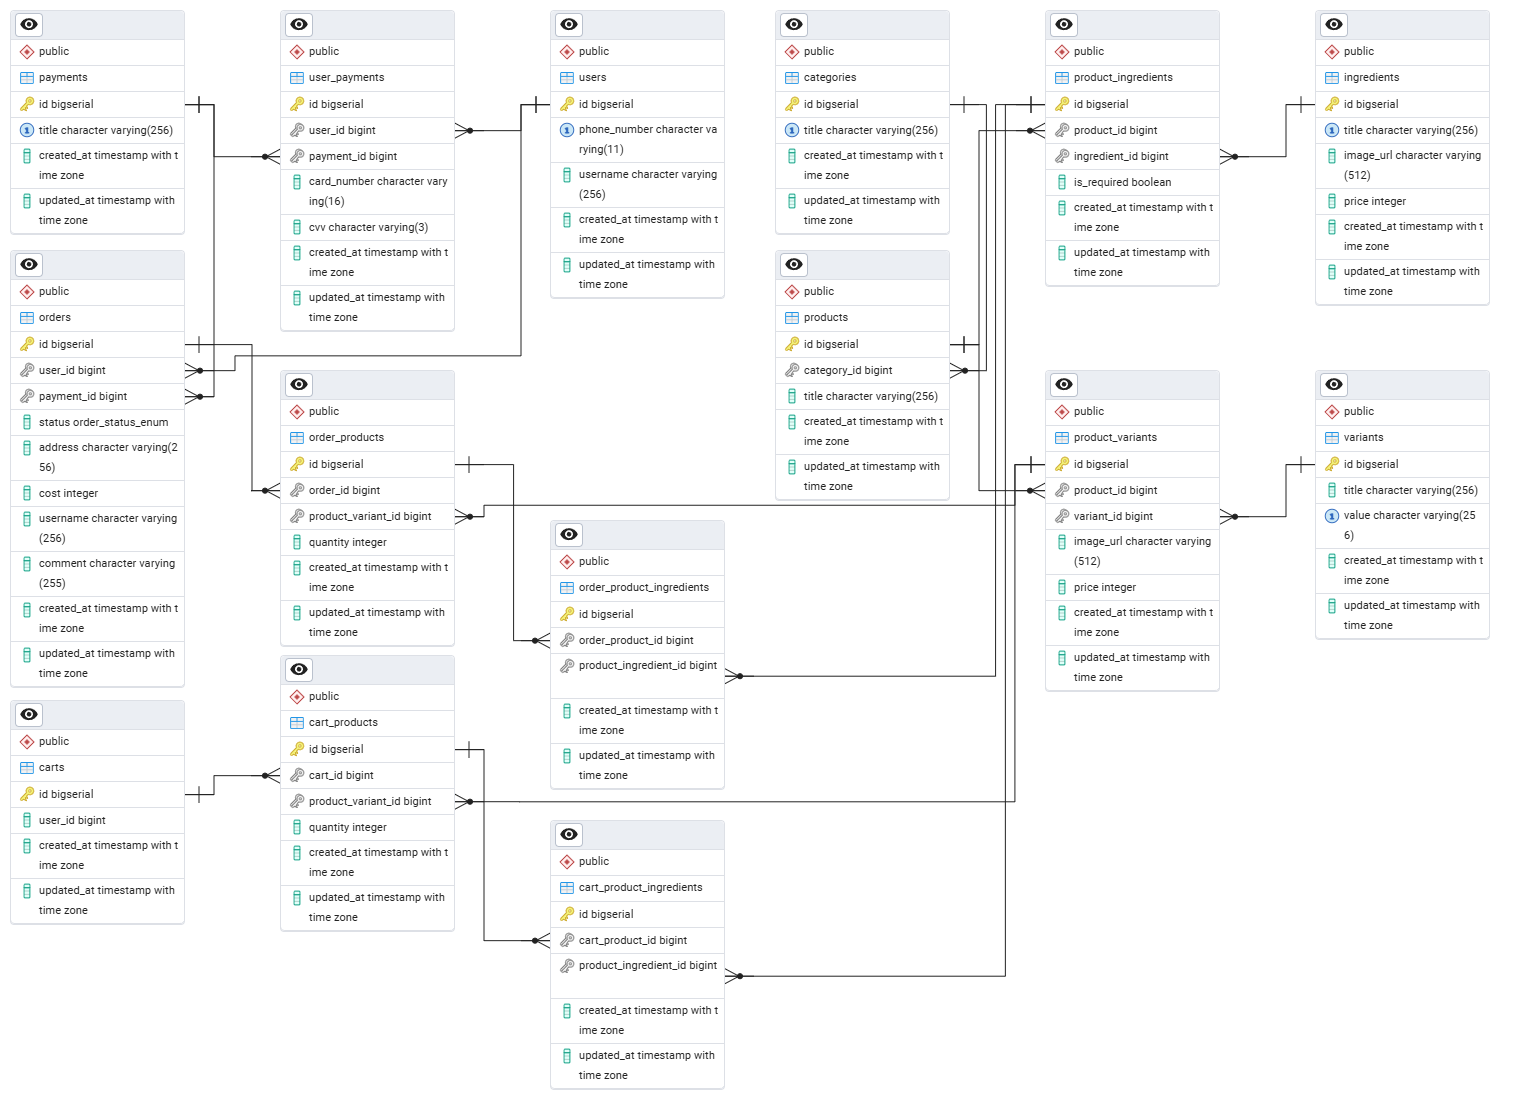
\includegraphics[width=1\linewidth]{img/er}
  \end{figure}
  \begin{center}
    Рисунок 1 – ER - диаграмма базы данных
  \end{center}

  SQL-скрипт для создания таблиц базы данных представлен ниже:

  \noindent
  \begin{Verbatim}[tabsize=4,fontsize=\small]
CREATE TABLE users (
    id BIGSERIAL PRIMARY KEY,
    phone_number VARCHAR(11) NOT NULL UNIQUE,
    username VARCHAR(256),
    created_at TIMESTAMP WITH TIME ZONE DEFAULT CURRENT_TIMESTAMP,
    updated_at TIMESTAMP WITH TIME ZONE DEFAULT CURRENT_TIMESTAMP
);

CREATE TABLE payments (
    id BIGSERIAL PRIMARY KEY,
    title VARCHAR(256) NOT NULL UNIQUE,
    created_at TIMESTAMP WITH TIME ZONE DEFAULT CURRENT_TIMESTAMP,
    updated_at TIMESTAMP WITH TIME ZONE DEFAULT CURRENT_TIMESTAMP
);

CREATE TABLE user_payments (
    id BIGSERIAL PRIMARY KEY,
    user_id BIGINT NOT NULL,
    payment_id BIGINT NOT NULL,
    card_number VARCHAR(16),
    cvv VARCHAR(3),
    created_at TIMESTAMP WITH TIME ZONE DEFAULT CURRENT_TIMESTAMP,
    updated_at TIMESTAMP WITH TIME ZONE DEFAULT CURRENT_TIMESTAMP,

    FOREIGN KEY (user_id) REFERENCES users(id) ON DELETE CASCADE,
    FOREIGN KEY (payment_id) REFERENCES payments(id) ON DELETE CASCADE
);

CREATE TABLE categories (
    id BIGSERIAL PRIMARY KEY,
    title VARCHAR(256) NOT NULL UNIQUE,
    created_at TIMESTAMP WITH TIME ZONE DEFAULT CURRENT_TIMESTAMP,
    updated_at TIMESTAMP WITH TIME ZONE DEFAULT CURRENT_TIMESTAMP
);

CREATE TABLE products (
    id BIGSERIAL PRIMARY KEY,
    category_id BIGINT NOT NULL,
    title VARCHAR(256) NOT NULL,
    description VARCHAR(512),
    created_at TIMESTAMP WITH TIME ZONE DEFAULT CURRENT_TIMESTAMP,
    updated_at TIMESTAMP WITH TIME ZONE DEFAULT CURRENT_TIMESTAMP,

    FOREIGN KEY (category_id) REFERENCES categories(id) ON DELETE RESTRICT
);

CREATE TABLE ingredients (
    id BIGSERIAL PRIMARY KEY,
    title VARCHAR(256) NOT NULL UNIQUE,
    image_url VARCHAR(512) NOT NULL,
    price INT NOT NULL CHECK (price >= 0),
    created_at TIMESTAMP WITH TIME ZONE DEFAULT CURRENT_TIMESTAMP,
    updated_at TIMESTAMP WITH TIME ZONE DEFAULT CURRENT_TIMESTAMP
);

CREATE TABLE product_ingredients (
    id BIGSERIAL PRIMARY KEY,
    product_id BIGINT NOT NULL,
    ingredient_id BIGINT NOT NULL,
    is_required BOOLEAN NOT NULL DEFAULT FALSE,
    created_at TIMESTAMP WITH TIME ZONE DEFAULT CURRENT_TIMESTAMP,
    updated_at TIMESTAMP WITH TIME ZONE DEFAULT CURRENT_TIMESTAMP,

    FOREIGN KEY (product_id) REFERENCES products(id) ON DELETE RESTRICT,
    FOREIGN KEY (ingredient_id) REFERENCES ingredients(id) ON DELETE RESTRICT
);

CREATE TABLE product_variants (
    id BIGSERIAL PRIMARY KEY,
    product_id BIGINT NOT NULL,
    image_url VARCHAR(512) NOT NULL,
    size INT CHECK (size > 0),
    volume INT CHECK (volume > 0),
    weight INT NOT NULL CHECK (weight > 0),
    price INT NOT NULL CHECK (price >= 0),
    created_at TIMESTAMP WITH TIME ZONE DEFAULT CURRENT_TIMESTAMP,
    updated_at TIMESTAMP WITH TIME ZONE DEFAULT CURRENT_TIMESTAMP,

    FOREIGN KEY (product_id) REFERENCES products(id) ON DELETE RESTRICT
);

CREATE TABLE carts (
    id BIGSERIAL PRIMARY KEY,
    user_id BIGINT NOT NULL,
    created_at TIMESTAMP WITH TIME ZONE DEFAULT CURRENT_TIMESTAMP,
    updated_at TIMESTAMP WITH TIME ZONE DEFAULT CURRENT_TIMESTAMP
);

CREATE TABLE cart_products (
    id BIGSERIAL PRIMARY KEY,
    cart_id BIGINT NOT NULL,
    product_variant_id BIGINT NOT NULL,
    quantity INT NOT NULL DEFAULT 1 CHECK (quantity >= 1),
    created_at TIMESTAMP WITH TIME ZONE DEFAULT CURRENT_TIMESTAMP,
    updated_at TIMESTAMP WITH TIME ZONE DEFAULT CURRENT_TIMESTAMP,

    FOREIGN KEY (cart_id) REFERENCES carts(id) ON DELETE RESTRICT,
    FOREIGN KEY (product_variant_id) REFERENCES product_variants(id)
      ON DELETE RESTRICT
);

CREATE TABLE cart_product_ingredients (
    id BIGSERIAL PRIMARY KEY,
    cart_product_id BIGINT NOT NULL,
    product_ingredient_id BIGINT NOT NULL,
    created_at TIMESTAMP WITH TIME ZONE DEFAULT CURRENT_TIMESTAMP,
    updated_at TIMESTAMP WITH TIME ZONE DEFAULT CURRENT_TIMESTAMP,

    FOREIGN KEY (cart_product_id) REFERENCES cart_products(id)
      ON DELETE RESTRICT,
    FOREIGN KEY (product_ingredient_id) REFERENCES product_ingredients(id)
      ON DELETE RESTRICT
);

CREATE TYPE ORDER_STATUS_ENUM AS ENUM (
    'pending', 'succeeded', 'canceled'
);

CREATE TABLE orders (
    id BIGSERIAL PRIMARY KEY,
    user_id BIGINT NOT NULL,
    payment_id BIGINT NOT NULL,
    status ORDER_STATUS_ENUM DEFAULT 'pending',
    address VARCHAR(256) NOT NULL,
    cost INT NOT NULL CHECK (cost >= 0),
    comment VARCHAR(255),
    created_at TIMESTAMP WITH TIME ZONE DEFAULT CURRENT_TIMESTAMP,
    updated_at TIMESTAMP WITH TIME ZONE DEFAULT CURRENT_TIMESTAMP,

    FOREIGN KEY (user_id) REFERENCES users(id) ON DELETE CASCADE,
    FOREIGN KEY (payment_id) REFERENCES payments(id) ON DELETE CASCADE
);

CREATE TABLE order_products (
    id BIGSERIAL PRIMARY KEY,
    order_id BIGINT NOT NULL,
    product_variant_id BIGINT NOT NULL,
    quantity INT NOT NULL CHECK (quantity >= 1),
    created_at TIMESTAMP WITH TIME ZONE DEFAULT CURRENT_TIMESTAMP,
    updated_at TIMESTAMP WITH TIME ZONE DEFAULT CURRENT_TIMESTAMP,

    FOREIGN KEY (order_id) REFERENCES orders(id) ON DELETE RESTRICT,
    FOREIGN KEY (product_variant_id) REFERENCES product_variants(id)
      ON DELETE RESTRICT
);

CREATE TABLE order_product_ingredients (
    id BIGSERIAL PRIMARY KEY,
    order_product_id BIGINT NOT NULL,
    product_ingredient_id BIGINT NOT NULL,
    created_at TIMESTAMP WITH TIME ZONE DEFAULT CURRENT_TIMESTAMP,
    updated_at TIMESTAMP WITH TIME ZONE DEFAULT CURRENT_TIMESTAMP,

    FOREIGN KEY (order_product_id) REFERENCES order_products(id)
      ON DELETE RESTRICT,
    FOREIGN KEY (product_ingredient_id) REFERENCES product_ingredients(id)
      ON DELETE RESTRICT
);
  \end{Verbatim}

  \section*{Вывод}
  В ходе выполнения лабораторной работы освоены схемы, пользователи и роли в PosgreSQL, изучены типы данных в PosgreSQL, освоены основные варианты DDL-запросов, закреплены знания по проектированию структуры реляционной базы данных. В результате выполнения разработана база данных для сервиса по доставке еды.

\end{document}